%\PassOptionsToPackage{unicode=true}{hyperref} % options for packages loaded elsewhere
%\PassOptionsToPackage{hyphens}{url}
%
\documentclass[a4paper,14pt,openany,final]{extreport} % с экрана надпись надо убрать
%\usepackage[times,fancytop,firamono,cpcaption,microtyping]{subook}
\usepackage[times,firamono,microtyping,irnitu,732,asanamath,smalltitles]{subook} % 732,asanamath
%\usepackage{booktabs}
\usepackage{multicol}
\usepackage{totcount}
\usepackage{multirow}
\usepackage{array}
\usepackage{makecell}
\usepackage{titlesec}
\usepackage{enumitem}
%\usepackage{tocloft}
\graphicspath{{./pics/}}
\renewcommand{\chaptername}{}
\makeatletter
\makeatother

%\usepackage{color}
%\usepackage{soul}
\date{}
% \hypersetup{
%     bookmarks=true,         % show bookmarks bar?
%     unicode=true,           % non-Latin characters in Acrobat’s bookmarks
%     pdftoolbar=true,        % show Acrobat’s toolbar?
%     pdfmenubar=true,        % show Acrobat’s menu?
%     pdffitwindow=false,     % window fit to page when opened
%     pdfstartview={FitH},    % fits the width of the page to the window
%     pdftitle={Компьютерные науки, часть 4},    % title
%     pdfauthor={Евгений Александрович Черкашин},     % author
%     pdfsubject={Методическое пособие},   % subject of the document
%     pdfcreator={EMACS-24.4:AuCTeX},   % creator of the document
%     pdfproducer={LuaLaTeX}, % producer of the document
%     pdfkeywords={Искусственный интеллект} {Логическое
%       программирование} {Планирование действий} {Удовлетворение
%       ограничений} {Компьютерная алгебра} {Принцип максимума} {Оптимальное управление}, % list of keywords
%     pdfnewwindow=true,      % links in new window
%     colorlinks=true,       % false: boxed links; true: colored links
%     linkcolor=[rgb]{0 0.4 0.1},          % color of internal links (black)
%     citecolor=blue,        % color of links to bibliography
%     filecolor=black,      % color of file links
%     urlcolor=[rgb]{0.3 0.0 0.3}           % color of external links
%   }

% \let\oldcaption\caption
%\renewcommand{\caption}[1]{\stepcounter{lastfig}\label{LastFig}\oldcaption{#1}}

\newcommand\theyear{2018}

\usepackage{xcolor}
\usepackage{stackengine}
\setstackgap{L}{.5\baselineskip}
\newcommand\MA[2]{{\sffamily\color{red}\hsmash{$\uparrow$}%
  \smash{\toplap{#1}{\scriptsize\bfseries #2}}}}
\newcommand\MB[2]{{\sffamily\color{red}\hsmash{$\downarrow$}%
    \smash{\bottomlap{#1}{\scriptsize\bfseries#2}}}}
\usepackage{tikz}

\newcommand*{\hl}[1]{%
\tikz[baseline]\node[rectangle, fill=yellow, rounded corners, inner sep=0.3mm,anchor=base]{#1};%
}
\makeatletter
   \def\vhrulefill#1{\leavevmode\leaders\hrule\@height#1\hfill \kern\z@}
\makeatother

\newcommand\toprule{\noindent\vhrulefill{2pt}}
\newcommand\bottomrule{\noindent\vhrulefill{2pt}}
\newcommand\midrule{\noindent\vhrulefill{2pt}}

\newtotcounter{captionsnum}
\def\oldcaption{} \let\oldcaption=\caption
\def\caption{\stepcounter{captionsnum}\oldcaption}

\newtotcounter{bibitemnum}
\def\oldbibitem{} \let\oldbibitem=\bibitem
\def\bibitem{\stepcounter{bibitemnum}\oldbibitem}

\newtotcounter{appsnum}
\setcounter{appsnum}{1}

\newcommand\T{\rule{0pt}{2.6ex}}       % Top strut
\newcommand\B{\rule[-1.2ex]{0pt}{0pt}} % Bottom strut
\newcommand{\BA}[1]{%
  \begin{minipage}[b]{0.4\textwidth}
    \raggedright\T
    #1
  \end{minipage}
}
\let\BT\BA
\newcommand{\BB}[1]{%
  \begin{minipage}[t]{0.4\textwidth}
    \raggedright\T
    #1
  \end{minipage}
}
\newcommand{\BC}[2]{%
  \begin{minipage}[c]{#1}
    \raggedright\T
    #2
  \end{minipage}
}

\makeatletter
\renewcommand\bibsection{%
\chapter{\bibname}%
\@mkboth{\MakeUppercase{\bibname}}{\MakeUppercase{\bibname}}%
}%
\makeatother


% Убрать марки и выделения.
\providecommand\hl[1]{}
\renewcommand\hl[1]{#1}
\renewcommand\MA[2]{}
\renewcommand\MB[2]{}
\renewcommand{\bibname}{Список использованных источников}
\providecommand\sfcpshape{\rmfamily}
\newcommand{\capfont}{\Large\sffamily\sfcpshape\bfseries}
\usepackage{pifont}

% setup list parameters
\setlist{itemsep=0pt plus 0.1pt,topsep=0pt plus 0.3pt,parsep=0pt plus 0.7pt}
\setlist[itemize]{label=\ding{113}}

\begin{document}
\renewcommand{\bibname}{СПИСОК ИСПОЛЬЗОВАННЫХ ИСТОЧНИКОВ}
\renewcommand{\chaptername}{}
\clubpenalty=10000
\widowpenalty=10000
\parskip=0pt plus 1pt

\tableofcontents

\chapter*{ВВЕДЕНИЕ}

Каждый человек рано или поздно сталкивается с проблемой выбора на рынке недвижимости.  Принимаемые в это время решения з значительно влияют на дальнейшую жизнь семьи, организации, фирмы и т.д.
Поэтому всякая помощь на этом этапе представляется необходимым моментом.  Для поддержи принятия решения существует целая индустрия -- услуги риелторов, задач которых организовывать процесс поиска интересующих объектов недвижимости на рынке, обеспечение безопасности сделки, соответствующий документооборот.

С другой стороны, на рынке недвижимости Иркутской области находятся много различных уникальных объектов, которые уже долгое время не могут найти себе рачительного хозяина, способного эффективно эту собственность ввести в эксплуатацию.  Как следствие, продавцы терпят убытки, платя налоги за нерентабельную собственность, а у покупателей нет возможности инвестировать свободные капиталы.  Причина такой ситуации -- неразвитость информационного обеспечения, т.е. несмотря на активную рекламу таких объектов риелторским конторам не удается найти покупателя.

Деятельность риелторов в некоторой степени автоматизируется.  Офисные пакеты используются для подготовки документации, ведется бухгалтерия, а также существуют сетевое программное обеспечение, которое организует и регламентирует взаимоотношения риелторов друг с другом, и с сервисами услуг оценки объектов и рынка недвижимости в целом.  При помощи таких CRM организуются сделки между риелторами: на некоторую плату объект передается другому риелтору на продажу, -- контроль ранних договоренностей.

С другой стороны, согласно рекламе сайта Avito, каждая вторая квартира продается именно через интернет--сайты без участия риелторов.  Опрос риелторов показал, что это не совсем так.  Многое зависит от <<традиций>> того или иного региона Российской Федерации.  Например, в Иркутской области и Москве недвижимость предпочитают продавать через интернет"=сайты, причем делается несколько предложений одной и той же квартиры на нескольких сайтах.  Опыт показывает, что это практически всегда приводит к тому, что цена на объект недвижимости падает ниже рыночной.  В Екатеринбурге, наоборот, недвижимость преимущественно продается через риелторские конторы, что и стабилизирует цены на жилье, и делает процесс купли"=продажи более предсказуемым для продавца.

В таблице \ref{tab:market-irk} представлены количественные характеристики роста рынка недвижимости Иркутской области.. В период с 2010 по 2016 год количество сделок только по жилой недвижимости на вторичном рынке выросло примерно на 20\%. Ежегодно в Иркутской области вводится в эксплуатацию не менее 30~000 новых квартир.
На сайте Avito.ru выставлены на продажу более 5~000 квартир, находящихся на территории Иркутской области.

\begin{table}[htb]
  \caption{Характеристика рынка недвижимости Иркутской области}
  \label{tab:market-irk}
  \centering
  \begin{tabular}{|c|c|}
    \hline
Год &
      Количество сделок \\
    \hline
2010 &
12594 \\
2011 &
13756 \\
2012 &
15080\\
2013 &
14540\\
2014 &
15651\\
2015 &
15005\\
2016 &
       15982\\
    \hline
\end{tabular}
\end{table}

Таким образом, для гармонизации процессов на рынке недвижимости имеет смысл разработать информационную систему, которая не только бы сообщала актуальную информацию об объектах недвижимости, но и помогала бы искать такие объекты покупателям.  Такой сервис должен функционировать на основе современных методов анализа и структуризации данных: выбирать для конкретных пользователей объекты недвижимости, которые потенциально могил бы его заинтересовать.  Такими системами в разных предметных областях выступают \emph{рекомендательные системы} (РС).

Рекомендательные системы \cite{b1} -- информационные систем поддержки принятия решений, предназначенные для оценки уровня интереса пользователя к определенному продукту или сервису объекту на основе имеющейся информации о пользователе и/или объекте. Отрасль разработки РС начала активно развиваться при появлении онлайн"=сервисов продаж, и в настоящее время РС – одно из активных направлений развития систем поддержки принятия решений, ориентированное, прежде всего, на коммерческое использование, а также на решение задач повышения продуктивности поиска релевантной информации.

В коммерции РС позволяют решать задачи установления, что именно представляет ценность для потребителя в виде набора конкретных объектов (например, товаров или услуг), сужение вариантов выбора и предоставление схожих вариантов других объектов, тем самым упрощая выбор. РС позволяют также выявлять новые характеристики объектов, например, при помощи ведения классификаций объектов и анализа набора известных признаков. Использование РС позволяет отделам снабжения коммерческих фирм-поставщиков предоставлять уникальный сервис каждому потребителю, увеличивая его доверие и лояльность к поставщику, увеличивая продажи и конверсию, а также получая и накапливая больше знаний о потребителях.

Рекомендательные системы появились в интернете достаточно давно, около 20 лет назад. Однако настоящий подъем в этой области случился примерно 5-10 лет назад, когда произошло соревнование Netflix Prize. Компания Netflix тогда давала в прокат не цифровые копии, а рассылала VHS-кассеты и DVD. Для них было очень важно повысить качество рекомендаций. Чем лучше Netflix рекомендует своим пользователям фильмы, тем больше фильмов они берут в прокат. Соответственно, растет и прибыль компании. В 2006 году они запустили соревнование Netflix Prize. Они выложили в открытый доступ собранные данные: около 100 миллионов оценок по пятибалльной шкале с указанием ID проставивших их пользователей. Участники соревнования должны были как можно лучше предугадывать, какую оценку поставит определенному фильму тот или иной пользователь. Качество предсказания измерялось при помощи метрики RMSE (средне-квадратичное отклонение). У Netflix уже был алгоритм, который предсказывал оценки пользователей с качеством 0.9514 по метрике RMSE (см.~раздел~\ref{sec:rs-eval}). Задача была улучшить предсказание хотя бы на 10\% — до 0.8563. Победителю был обещан приз в \$1~000~000. Соревнование длилось примерно три года. За первый год качество улучшили на 7\%, дальше все немного замедлилось. Но в конце две команды с разницей в 20 минут прислали свои решения, каждое из которых проходило порог в 10\%, качество у них было одинаковое с точностью до четвертого знака. В задаче, над которой множество команд билось три года, все решили каких-то двадцать минут. Опоздавшая команда (как и многие другие, участвовавшие в конкурсе) остались ни с чем, однако сам конкурс очень сильно подстегнул развитие в этой области [2].

% TODO: Цели, задачи, требования

\paragraph{Целью}\hspace{-1em} данной выпускной квалификационной работы магистранта является проектирование и реализация рекомендательной системы для рынка недвижимости Иркутской области, применимой для решения перечисленных выше проблем.

Для достижения цели \textbf{решены следующие задачи}:
\begin{enumerate}
\item Анализ предметной области рекомендательных систем и рынка недвижимости;
\item Тестирование разработанной рекомендательной системы.
\end{enumerate}

К создаваемому программному обеспечению выдвигались следующие дополнительные \textbf{требования}:
\begin{enumerate}
\item система должна вырабатывать рекомендации в режиме <<холодного старта>>;
\item не принуждать пользователей к регистрации и авторизации, но при этом обеспечивать накопление необходимой информации;
\item тестирование системы должно производится на данных рынка недвижимости Иркутской области, что обеспечивает экспертную оценку рекомендаций;
\item программное обеспечение необходимо реализовать преимущественно на свободных (\foreignlanguage{english}{open-source)}) технологиях.
\end{enumerate}

\chapter{Технологии разработки информационных интернет"=систем}
\label{chap:dev-tech-theory}

В данном разделе рассматриваются технологии, которые использованы для проектирования и реализации рекомендательной системы для рынка недвижимости Иркутской области.

\section{Рекомендательные системы}
\label{sec:domain-descr}

В области рекомендательных систем используется специальная терминология. \emph{Объектом} обозначается то, что система рекомендует \emph{пользователям}, например, продукты, услуги, товары, новости, книги, DVD и т.п. \emph{Профилем пользователя} или \emph{объекта} являются данные, характеризующие пользователя или объект. Именно эти данные используются в процессе оценивания \emph{релевантности} объекта к желаниям пользователя. Этот процесс называется \emph{фильтрацией} (\foreignlanguage{english}{filtering}). В результате фильтрации объекты \emph{ранжируются} в соответствии с полученной оценкой, а пользователю предоставляется некоторое конечное подмножество, элементы которого имеют максимальную релевантность, т.е. оцениваются как наиболее интересные пользователю. Далее под \emph{интересом} будем понимать именно интерес пользователя к объекту. Т.к. РС -- это, прежде всего, информационные системы, то все объекты и пользователи описываются при помощи \emph{атрибутов}. Именно атрибуты являются входной информацией во все процедуры оценивания интереса. \emph{Качество рекомендации} -- оценка точности предсказания интереса, сделанного РС, например, в сравнении с имеющимися примерами, т.е. оценками конкретных объектов конкретными пользователями.

Рекомендательные системы полезны не только для информационных ресурсов и порталов электронной коммерции, но и могут также открыть новые возможности в области безопасности, автомобильной промышленности [3], рекламе [4] и др.
Существует ряд подходов к оценке интереса.

Существует ряд подходов к оценке интереса:
\begin{enumerate}
\item на основе \emph{фильтрации содержания}
  (\foreignlanguage{english}{content-based information filtering}), при этом в информационной
  системе создаются профили пользователей и объектов, включающие
  социальный статус пользователя, возраст, место проживания, род
  деятельности, а также характеристики, выражающие интерес
  пользователя к объекту; профили объектов включают позицию в системе
  классификации, его потребительские характеристики. % вакханалия
\item	на основе\emph{ коллаборативной фильтрации} (\foreignlanguage{english}{collaborative filtering}), где используется информация о поведении пользователей в прошлом, например, перечень покупок или оценок объектов, сделанных на сайте интернет-магазина в прошлом пользователями из той же группы интересов, при этом аналитическим блоком информационной системы автоматически формируются классификации объектов, производится \emph{ранжирование атрибутов} по степени значимости в оценке интереса.
\item	\emph{интеллектные} (knowledge-based), где оценка вычисляется на основе формализованных знаний.
\item	\emph{гибридные} (\foreignlanguage{english}{hybridprediction}) методы, которые базируются на подходах пп. 1 и 2, включая элементы из 3, что призвано повышать эффективность 1 и/или 2.
\end{enumerate}

Например, в Music Genome Project музыкальный аналитик оценивает каждую композицию по сотням различных музыкальных характеристик, при помощи которых выявляются музыкальные предпочтения пользователя. Перечень оценок формирует \emph{профиль музыкального произведения}. Основная проблема первого типа РС (фильтрации содержания) — это работоспособность системы на начальном этапе ее эксплуатации, так называемый <<\emph{холодный старт}>>: для новых пользователей в системе нет необходимой информации в профиле для принятия решения о том, какие объекты следует предлагать. В связи с этим в современных рекомендательных системах реализуется механизм сбора и анализа данных о пользователях с применением \emph{явных} и \emph{неявных методов}.

Явные методы сбора данных выполняют следующие действия:
\begin{itemize}
\item запрос у пользователя оценки объекта по некоторой шкале;
\item запрос у пользователя ранжировки группы объектов от наилучшего к наихудшему;
\item предъявление пользователю двух объектов с вопросом о том, какой из них лучше;
\item предложение создать список объектов, характеризующих предпочтения пользователя.
\end{itemize}
Примерами неявного сбора данных выступают:

\begin{itemize}
\item наблюдение за тем, что просматривает пользователь в
  интернет-магазине или базе данных;
\item ведение записей о поведении
  пользователя онлайн.
\end{itemize}
Сбор информации из социальных сетей, например, как в [5-7].

Второй тип РС, основанные на коллаборативной фильтрации, сравнивают однотипные данные, полученные от разных людей и вычисляют список рекомендаций для конкретного пользователя. Для вычисления рекомендаций используется, например, граф интересов. Таким образом, РС представляют собой информационные системы, дополненные алгоритмами, позволяющими обнаружить в хранилище объекты, которые не имеют непосредственного отношения к запросу пользователя. Любопытно, что рекомендательные системы часто используют как поисковые машины для индексации необычных данных.

Более подробное описание различных подходов к реализации подсистем РС рассмотрим на примерах из современной литературы.

\section{Примеры использования РС}
\label{sec:rs-examples}

В обзоре \cite{b8} рассмотрены РС в области предоставления пользователям текстовых документов, в частности, научных статей. Больше половины (55\%, 34 из 62) систем построены на основе фильтрации содержания. Алгоритмы коллаборативной фильтрации использованы только в 18\% (11 из 62) случаев. Представлены подходы, основывающиеся на стереотипировании и гибридных методах. Авторы исследования пришли к выводу, что в 81\% случаев моделирование пользователя на основе автоматического сбора информации не приносит значимых результатов по сравнению с явным указанием набора ключевых слов.

В основе характеристик объектов, научных статей, в исследованных РС используют просто ключевые слова, содержащиеся в документах, реже \(N\)-граммы, а также нетекстовые элементы, такие как ссылки на другие статьи и фамилии авторов. Самая популярная модель для хранения представления статей -- модель векторного пространства. Моделирование пользователя осуществляется при помощи графов и списков тем, назначенных пользователям в результате машинного обучения. Темы объединяются в иерархические справочники, например, на основе классификаторов АСМ. В рассмотренных подходах тексты извлекаются из заглавий, аннотаций, заголовков, введения, предисловия, предоставленных автором ключевых слов, библиографии, основного текста, социальных тегов и цитирований контекста.

В РС, где применялась коллаборативная фильтрация, и ни в одном из проектов не удалось успешно использовать явные рейтинги: пользователи были слишком ленивы, чтобы самостоятельно задавать рейтинг статьям. Неявные рейтинги получены из данных по количеству страниц, прочитанных пользователем, взаимодействию пользователей с документами (загрузка, редактирование, представление) и цитирования. Главная проблема коллаборативной фильтрации для научных работ -- это дефицит информации, например, для РС научных статей Mendeley по сравнению с Netflix (онлайн фильмы) дефицит составляет три порядка.  Неявные рейтинги объектов получаются из анализа одновременной загрузки статьи (со"=загрузка) разными пользователями одной группы, совместного просмотра (со"=просмотр), совместное цитирование статьями (со"=цитирование) одних и тех же источников. Оказалось, что со"=цитирование, будучи эффективным в начале появления статьи на сервисе РС, через два года начинает уступать со"=загрузке. Популярным подходом представления результата такого анализа являются графы. Вершины графа -- это статьи, представленные наборами атрибутов, а дуги -- соотношения между статьями.

Основными проблемами в области РС являются следующие:
\begin{itemize}
\item отсутствие общего базиса оценивания качества систем (по
  предметным областям), включая объективную информацию о реальных
  оценках реальных пользователей, нестабильность методов оценивания и
  высокая их зависимость от <<шума>>;
\item неиспользованный потенциал
  научных исследований: новые научные результаты не внедряются в
  практические приложения (большинство работающих РС базируются на
  простых методах), данные существующих практических реализаций РС
  научно не исследуются, нет тесного взаимодействия со снежными
  областями анализа данных, а так же друг с другом, низкий научный
  интерес к РС;
\item в оценке удовлетворенности не учитывается факторы
  конфиденциальность, безопасности данных, разнообразие, разметка и
  презентация информации; в значимом количестве РС моделирование
  пользователя было крайне примитивно - набор ключевых слов,
  собственная статья или просто фрагмент текста, представляющих
  научные интересы пользователя.
\end{itemize}
    Среди открытых проектов выделяются MyMediaLite, LensKit, Mahout, Duine, RecLabCore, Easyrec и Recommender.

\subsection{Методы фильтрации содержания}
\label{sec:content-filtering}

В статье \cite{b5} решается задача анализа профиля пользователя в социальной сети ВКонтакте для решения проблемы холодного старта в решении задачи рекомендации жанров и произведений музыки и фильмов. Авторами разработана РС «EZSurf» автоматизирующая процесс веб"=сёрфинга и фильтрации контента, используя профиль пользователя в социальной сети <<ВКонтакте>>, а также API сервисов last.fm, TheMovieDB для получения сведений о схожих объектах (музыкальных произведений). Такой подход существенно упрощает хранилище данных РС, поскольку не требует создания собственной системы классификаций и базы объектов.

В статье \cite{b9} рассматривается задача выделения $N$ объектов с наивысшими оценками интереса, задача top"=$N$, при применении фильтрации контента. Предлагается математическая модель контентной рекомендательной системы, основанная на нечетких множествах, критерий оценки качества рекомендаций и алгоритм решения задачи. Математическая модель и алгоритм протестированы на данных сайта last.fm.

\subsection{Методы коллаборативной фильтрации}
\label{sec:collab-filtering}

Подходы, основанный на коллаборативной фильтрации, в настоящее время более популярны, чем подходы на основе фильтрации содержимого, вероятно из-за того, что представляет собой отражение практического опыта: большинство коммерческих РС вынуждены решать проблему недостатка информации, <<холодный старт>>, а также адаптируемости существующих сообществ пользователей к новым объектам.

Суть идеи коллаборативной фильтрации изображена на рисунке~\ref{fig:collab-essence}. Пользователям предоставляются интересующие их товары, которые они оценивают «положительно» или «отрицательно» пока пользуются сайтом, например, интернет"=магазином.

\begin{figure}[htb]\centering
  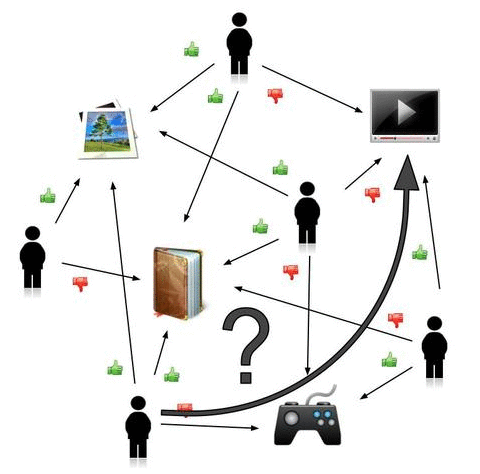
\includegraphics[width=0.5\linewidth]{collab1.png}
\caption{Накопление рейтингов покупателей о товарах}
\label{fig:collab-essence}
\end{figure}

Накопленные данные записывается в таблицу, которая представлена на рисунке~\ref{fig:collab2}, где столбцы -- это объекты, т.е. товары, а строки -- это оценки пользователей.
\begin{figure}[htb]
  \centering
  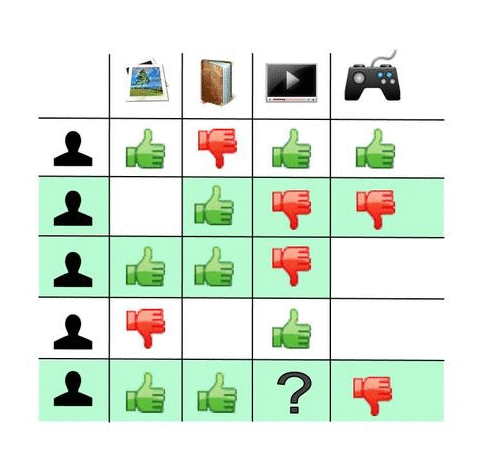
\includegraphics[width=0.5\linewidth]{collab2.png}
  \caption{Таблица собранной информации об оценках товаров пользователями}
  \label{fig:collab2}
\end{figure}

Задача рекомендательной системы, заключается в заполнение <<всех>> ячеек, помеченных вопросительным знаком на рисунке~\ref{fig:collab2}.

Для оценки интереса пользователя к объекту, помеченному вопросительным знаком, сравниваем пятого (последнего) пользователя со всеми остальными пользователями по критерию схожести его выбора. Пользователи под номерами «пять» и «три», схожи по первым двум товарам, т.к. оба ответили «положительно» по данным товарам. Пользователи под номерами «пять» и «два», схожи по товарам под номерами «два» и «четыре», т.к. оба ответили одинаково «положительно» на товар под номером «два» и «отрицательно» под номером «четыре». Следовательно, можно предположить, что пользователь под пятым номером скорее всего отнесется «отрицательно» к товару под номером «три», что представлено на рисунке~\ref{fig:collab3}.

\begin{figure}[htb]
  \centering
  
\includegraphics[width=0.5\linewidth]{collab3.png}
  \caption{Пример рекомендации}
  \label{fig:collab3}
\end{figure}

	Полученная оценка означает, что пользователю данный товар будет показываться в последнюю очередь.


Математические обозначения элементов модели сравнения состоит из набора пользователей $U$  и набора объектов $O$. Тогда $O_u$ -- это множество элементов, оцененных пользователем $u$, $U_0$ -- множество пользователей, которые оценили объект $o$, $r_{u,o}$ -- оценка пользователя $u$ для объекта $o$, $\mathbf{r}_u$ -- вектор всех оценок пользователя $u$, $\mathbf{r}_o$  -- вектор всех оценок объекта $o$, $\bar{r}_u$ и $\bar{r}_o$ -- средние значения оценок пользователя $u$ и объекта $o$,   соответственно. Сравнительная оценка обозначается $\hat{r}_{u,i}$. Для задания этой оценки сначала задается мера близости объекта $i$ к объекту $j$. Рассмотрим несколько популярных вариантов оценки близости.

Коэффициент Пирсона [3]:
\[
  s_{i,j}=\frac{\sum\limits_{u\in U}(r_{u,j}-\bar{r}_i)(r_{u,j}-\bar{r}_j)}{\sqrt{\sum\limits_{u\in U}(r_{u,j}-\bar{r}_i)^2}\sqrt{\sum\limits_{u\in U}(r_{u,j}-\bar{r}_j)^2}}
\]
где $U=U_i\cup U_j$ -- множество пользователей, которые оценили объекты $i$ и $j$.

Косинус угла между двумя векторами $\mathbf{r}_i$ и $\mathbf{r}_j$:
\[
  s_{i,j}=\cos(\mathbf{r}_i,\mathbf{r}_j)=\frac{\mathbf{r}_i \cdot \mathbf{r}_j}{|\mathbf{r}_i||\mathbf{r}_j|}.
\]
Затем производится формирование конечного множества объектов $S$ наиболее близких к объекту $o$. Вычисление рейтинга объекта $o$ делается по формуле:
\[
  \hat{r}_{u,o}=\frac{\sum\limits_{j\in S}S_{o,j}\cdot r_{u,j}}{\sum\limits_{j\in S}|S_{o,j}|}.
\]

Популярный подход к формированиюмножества рекомендаций -- это упорядочивавшие всех объектов по критерию схожести и выборке некоторого фиксированного количества объектов с максимальным рейтингом [Нефедова]. В качестве меры схожести (\foreignlanguage{english}{similarity}) двух объектов выступает $\cos$ угла между $N$-мерными векторами.

В [3,10] так же представлен обзор способов использования вышеупомянутых методов вычисления оценок, которые разделены на два класса -- \emph{анамнестические}, т.е. основывающиеся на одновременной обработке всех имеющихся данных, и \emph{модельные}, где производится предварительная обработка данных, выполняемая, например, раз в сутки. Второй класс позволяет быстрее вычислять оценки интереса, однако не обеспечивает актуальности данных. В классе аналитических способов, как правило, используются методы многомерного анализа данных на основе <<ближайшего соседства>> (\foreignlanguage{english}{Neighbourhood-based}), в то время как в модельных методах используется методы анализа скрытых факторов (\foreignlanguage{english}{Latenet Factors}). Существуют гибридные методы, объединяющие оба предыдущих класса.

\subsection{Метод Slope One}

Одним из интересных достижений в области РС является изобретение метода коллаборативной фильтрации <<Slope One>> \cite{slopeone}, разработанного в компании Amazon для формирования рейтинга товаров известного на весь мир магазина. Исследователи изучали факторы, приводящие к эффекту <<переобучения>>, т.е. нестабильному поведению системы при подаче на вход примерно одинаковых данных. В \cite{slopeone} предложено три схемы с формулой оценки вида $f(x)=x+b$ и предварительно вычисленном средней разнице рейтингов (оценок пользователей) двух объектов для всех пользователей, которые оценили оба эти объекта одновременно.  Здесь, $x$ -- известный рейтинг объекта, заданного (оцененного) некоторым пользователем, $b$ -- средняя разница рейтинга по всем пользователям для данного объекта, $f(x)$ -- оценка объекта для нового пользователя, т.е. пользователя, не задававшего какую-либо оценку для данного объекта.

Основное отличие данного алгоритма заключается в его простоте реализации, запросы к базе исходных данных также реализуются просто, алгоритм достаточно точен, а также алгоритм поддерживает и статический и динамический режим обновления промежуточных данных. То есть алгоритм позволяет создавать подсистемы оценки объектов для метода коллаборативной фильтрации для реально функционирующих систем.

Наглядно суть функционирования метода представлена на рисунке~\ref{fig:slope-exp} (рисунок адаптирован из оригинальной статьи \cite{slopeone}). Средняя разница в рейтинге товаров $o_1$ и $o_2$ по двум известным оценкам пользователя $u_1$ составляет $1.5-1 = 0.5$. Следовательно, если известно, что пользователь $u_2$ присвоил рейтинг товару $o_1$ рейтинг 2, то рейтинг товара $o_2$ составит $2+0.5=2+(1.5-1)=2.5$.

\begin{figure}[htb]
  \centering
  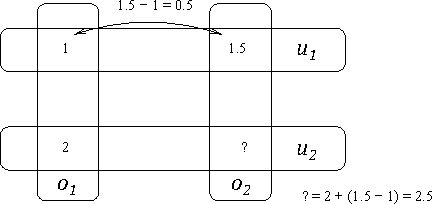
\includegraphics[width=0.7\linewidth]{slopeone.pdf}
  \caption{К объяснению работы алгоритма Slope One}
  \label{fig:slope-exp}
\end{figure}

При помощи данного алгоритма рейтинги объекта $o_2$, в общем случае, вычисляются из оценок нескольких пользователей и относительно разных объектов.  Т.е. получается несколько рейтингов одного и того же объекта. В этом случае считается средневзвешенная оценка полученных рейтингов, где в качестве весового коэффициента выступает количество раундов оценивания, другими словами, <<сколько раз пользователь $u_i$ проголосовал за <<опорный>> объект $o_j$?>>


\subsection{Гибридные методы}
\label{sec:hybrids}

В статье [11] рассмотрена задача разработки алгоритмов оценивания лекционного материала. Авторами предложен алгоритм вычисления близости лекций (объектов), где каждая лекция характеризуется подмножеством некоторого набора значений (например, подмножеством авторов лекций относительно множества всех авторов). Базовый алгоритм реализует подход фильтрации содержания. Для алгоритма подобранны коэффициенты, при помощи которых можно объединять оценки различных атрибутов в одну общую оценку лекции. Наиболее значимыми атрибутами оказались «категории», «авторы», «языки», «название» и «описание». Цель -- синтезировать набор лекций фиксированной длины, рекомендованных для просмотра заданному пользователю, из фиксированного множества <<новых>>, не использованных в построении профилей пользователя и объекта.

Далее алгоритм дополняется предсказателем последовательностей лекций: заданы примеры последовательностей из трех лекций, требуется для последовательностей из двух предложить третью, четвертую и т.д. Последовательности лекций приобретены системой неявно, т.е. фиксируя просмотренные пользователем лекции. Алгоритм занял первое место в соревновании, причем со значительным отрывом от второго места. Производится внедрение результатов исследований в области анализа сигналов и предсказания последовательностей событий.


%Приложения рекомендательных систем

    В \cite{b12} создан рекомендательный сервис новостей посетителям сайта, время пересчета рекомендаций в котором на каждую тысячу новых записей в журнале WEB"=сервера составляет 1.5--2 с., что авторами заявлено как ресурс, функционирующий в режиме, близком к реальному времени. Для проекта Рамблер"=новости подобный результат является удовлетворительным, так как 1000 новых запросов к сайту делается за чуть большее время. В исследовании использован адаптированный алгоритм MinHash для идентификации записей журнала и неточного их сравнения. Целью работы было показать целесообразность применения NoSQL"=технологий для создания сервисов указанного качества.

    Важным свойством приведенной реализации является то, что задачи хранения и анализа данных удалось объединить с задачей предоставления доступа к результатам в единой системе, избежав накладных расходов на перемещение данных из одного источника в другой, что улучшило общую производительность сервиса. Кроме того, предложенный подход упрощает решение повседневных задач сбора статистики о взаимодействии пользователя с веб"=приложением путем анализа структурированных логов мощным языком запросов СУБД MongoDB.  В результате продемонстрировано, что применение NoSQL к решению подобного класса задач является весьма перспективным.

\subsection{Оценка релевантности рекомендаций}
\label{sec:rs-eval}

Как и любая система структуризации информации РС оцениваются с точки зрения степени корректности расчетов рекомендаций. Классическим подходом является пример из \cite{b13}, где рассматривается задача сравнительной оценки различных подходов к построению РС.  Эта оценка, RMSE, среднеквадратическое отклонение, выполняется при помощи формулы:
    \[
      \mbox{RMSE}=\sqrt{\frac{1}{|D|}\sum_{(u,o)\in D}(\hat{r}_{u,o}-r_{u,o})^2},
    \]
где $D$ -- множество пар пользователей $u$ и объектов $o$, $r_{u,o}$ -- оценка интереса объекта $o$ пользователем $i$, \(\hat{r}_{u,o}\) -- оценка интереса, сделанная РС. Другие оценки представлены в \cite{b10}. % Nefedova




\section{РС для рынка недвижимости}
\label{sec:ex-retail}


В [18] предложен проект системы управления недвижимым имуществом, где варианты объектов предлагаются на основе вывода на прецедентах (case-based reasoning). Задача подсистемы вывода – найти  прецедент в базе имеющихся прецедентов, похожий на запрос пользователя. Система помогает покупателям найти имущество, соответствующее их запросам. При этом система выводит суждения о свойствах объектов. Полученная информация затем используется в процессе фильтрации содержания и коллаборативной фильтрации. В дополнение к полученному списку выводится также наиболее популярные (most visited) варианты.

В теоретическом исследовании [15] в системе пользователи разделены на продавцов и покупателей. Продавцы "рекламируют" свое имущество, выставленное на продажу, выделяя те свойства недвижимости, которые сами считают важными. Предложена идея того, как получать данные для фильтрации содержания в задаче разработки РС управления имуществом: продавцы выступают в виде экспертов-оценщиков недвижимости, формируя информационную базу для фильтрации содержания. Предложенную идею можно дополнить, если ввести третий класс пользователей - экспертов-риелторов и позволить им дополнять базу данных прецедентов новыми суждениями.

В [16] опытным путем показано, что использование Интернета не влияет значительно на эффективность поиска недвижимости с целью ее покупки по критериям времени поиска, его гибкости и "удовлетворенность результатом". Согласно исследованию Национальной ассоциации риелторов, проведенном в 2011 году, показано, что 88\% покупателей выбрали Интернет в качестве основного источника информации, но при этом среднее время на поиск жилья составило 12 недель, оно оказалось сравнимым с измерением, проведенным в 2009 году. Пользователь просматривает больше информации (как объектов, так и их свойств), но на анализ этой информации так же тратится много времени. Для повышения скорости выдачи результата авторами разработан алгоритм поиска на основе анализа поведения пользователей в процессе поиска объекта недвижимости, а также WEB-система, основанная на прецедентном выводе и онтологической концептуальной модели предметной области, ориентированная на пользователя.

В [23] авторами выделены три ключевые характеристики объекта недвижимости, которые в значительной мере является определяющими в процессе принятия решения – это "расположение" (location), "потребительская характеристика" (housing unit property) и "цена" (price). Большинство РС используют именно эти характеристики для фильтрации содержания, причем для критерия "потребительская характеристика" задаются формальные параметры объекта (площадь, номер этажа, количество балконов, комнат-спален и т.п.). На окончательное решение также влияет окружение объекта - расстояние до магазинов, школ, детских садов. Для того, чтобы учесть эти характеристики в [16] построена онтологическая модель, связывающая различные характеристики недвижимости в три древовидные структуры, описывающие варианты терминов "расположение", "потребительская характеристика" и "цена". Например, как вариант, под "расположением" понимается "расстояние" до места работы "пешком", выраженное в минутах. Так же "расположение" - это наличие в "окружении" (environment) объекта недвижимости "услуг" "фитнеса". При помощи онтологии получена возможность сравнивать не вполне "схожие" объекты, что повышает точность обработки информации.
Важным достижением авторов [16] является разработанный прототип РС, в котором пользователю предоставляется возможность указать на карте города область (окружность с заданным радиусом), в которой он хотел бы приобрести объект недвижимости, уточнить его потребительские характеристики и возможный диапазон цен.

Затем система выводит на карту варианты объектов недвижимости. Далее пользователь может уточнить другие характеристики, тем самым сужая количество предоставляемых вариантов. В сравнении с сервисами, подобным Avito.ru [17], пользователю предлагается меньше вариантов, т.е. система оценивает интерес пользователя более точно, и сильнее сужает количество альтернатив.
В [18] решается сложная логистическая задача организация процесса управления имуществом, в который вовлечены разнообразные группы людей в изменяющихся деловых и экономических условиях. В оценке учитываются не только экономические и бизнес-критерии, но и такие критерии, как "технологичность", "комфорт", "пространство", "административные" и "технические". Основная цель исследования - разработать модель, в которой различные группы людей будут максимально удовлетворены в "рациональной микро- и макро-среде".

Эффективность использования имущества предлагается оценивать по целой системе критериев, включающей цену объекта, цену владения этим объектом, цену ремонта, возможности его использования (capasity), количеству операций, которые необходимо выполнить по передаче собственности, надежность, комфорт, срок физической и технической эксплуатации, и др. Авторы разрабатывают математический аппарат для оценивания каждого объекта недвижимости – цены, эргономики, стоимости ремонта, назначение и т.п. Математическое обеспечение РС предложено развивать в направлении ухода от поиска <<наиболее экономически выгодного управления недвижимостью>> к мультикритериальному выбору и тем самым повысить эффективность вычислительных процессов.

% РС (анализа, оценки и т.п.).

Таким образом, на современном этапе развития РС важными вопросами, решаемыми в процессе проектирования РС объектов недвижимости являются:
\begin{itemize}
\item разработка концептуальной модели предметной области в виде
  онтологии;
\item создание математических моделей предсказания значений атрибутов, описывающих объект недвижимости;

\item реализация механизмов компьютерного обучения и логического вывода на основе прецедентов;

\item обеспечение информационного наполнения РС для оценки качественных атрибутов (например, наличия школ и магазинов в шаговой доступности).
\end{itemize}
Решение данных задач в значительной мере влияет на качество и точность предсказания оценки значимости объекта недвижимости для пользователя.

\subsection{Сопутствующие технические задачи}
\label{sec:co-tasks}

Одной из важных задач, решаемых при разработке РС, является создания пользовательского интерфейса, адекватно отображающего систему критериев, ко которым необходимо производить подбор объектов для пользователя. Например, в статье \cite{b14} представлен модуль естественно"=языкового интерфейса к базе данных РС, который реализован на основе математических моделей семантических объектов. При помощи модели решаются задачи определения семантики языковой конструкции, заданной пользователем, включая синонимы, классы, отношения и ограничения. В статье приводятся сведения о программной реализации предложенного метода в среде PHP~+~SQL и результатах тестирования программы на задаче доступа к базе данных РС автомобильного салона.

В \cite{b15} решается проблема обеспечения ограничения доступа к личным данным пользователей в контексте построения РС встраивания рекламных сообщений в информационный поток. При этом необходимо контролируемо предоставлять в одностороннем порядке в РС информацию из БД пользователей. Предложено вместо традиционных средств VPN (\foreignlanguage{english}{Virtual private network}) использовать режим функционирования сети с синхронным изменением IP"=адреса сервера и переключение клиента на этот адрес.

\paragraph{Выводы по разделу.}

Рекомендательные системы (РС) позволяют структурировать объекты в базе данных информационного ресурса (интернет-магазина) по степени релевантности к интересам того или иного пользователя (категории пользователей). Они позволяют решать задачи поиска новых закономерностей в таких данных, новые свойства и характеристики объектов.

РС активно применяются в интернет-магазинах, библиотеках текстового содержания (цифровых архивов статей научного учреждения или проекта, книг), а также на рынках недвижимости.

В области РС существует ряд фундаментальных и практических проблем, требующих решения как на этапе разработки РС, так и на этапе их эксплуатации:
\begin{itemize}
\item пользователи неохотно предоставляют информацию о себе и
  своих потребностях, либо разработчики РС уделяют мало внимания
  процессу информационного наполнения профиля пользователя;
\item в предметных областях, связанных с большой стоимостью объекта или услуги (где принимается серьезные решения по вложения материальных средств), информационные модели объекта и профиля пользователя сложны по своей структуре и связи компонент структуры, что требует явного представления концептуальной модели предметной области во время выполнения РС как своих основных функций, так и функций предсказания значений атрибутов объекта или профиля пользователя на основе прецедентов;
\item для предыдущего пункта важным является также разработка пользовательского интерфейса, позволяющего в удобной для пользователя форме и достаточно гибко задавать запросы к РС, а также визуализировать результаты, предлагаемые РС;
\item при практической реализации РС практически всегда необходимо решать проблему <<холодного старта>>, т.е. обеспечивать функционирование информационной системы в режиме недостатка исходных данных о предпочтениях пользователей.
\end{itemize}
Таким образом РС, как системы поддержки принятия решения, являются типичным представителем систем искусственного интеллекта, ориентированными, прежде всего, на обработку неполной и противоречивой информации, а также использующими системы, основанные на формализованных знаниях (\foreignlanguage{english}{knowledge-based systems}).


\chapter{Реализация рекомендательной систем для рынка недвижимости Иркутской области}
\label{chap:dev-tech-theory}

\begin{thebibliography}{99}
\bibitem[slopeone]{slopeone} Daniel Lemire, Anna Maclachlan. Slope One Predictors for Online Rating-Based Collaborative. [Электронный ресурс] URL:~\url{http://cogprints.org/4031/1/lemiremaclachlan_sdm05.pdf}.
\end{thebibliography}


\end{document}

%%% Local Variables:
%%% mode: latex
%%% TeX-master: t
%%% End:
